\begin{figure}[!htb]
\centering
\resizebox{\linewidth}{!}{%
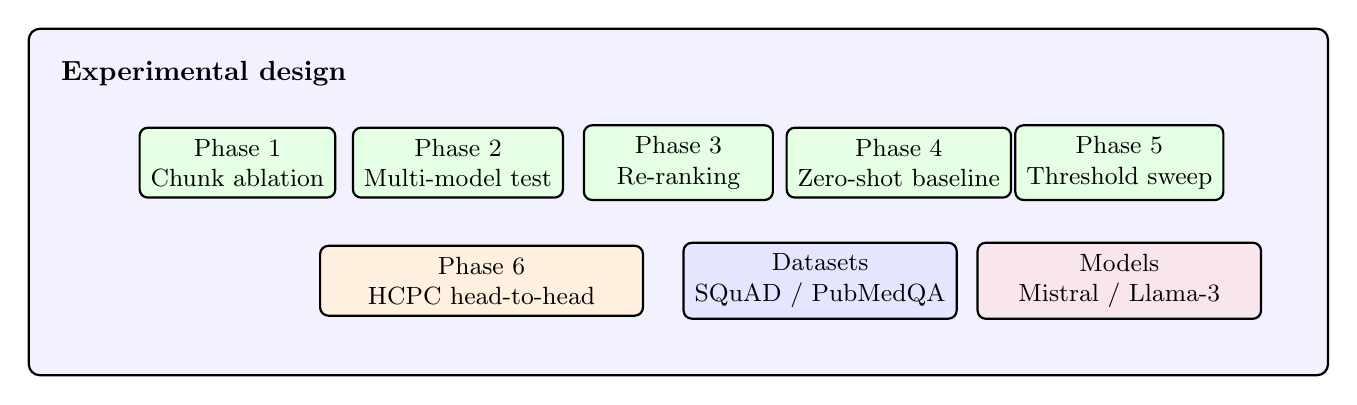
\begin{tikzpicture}[
  font=\small,
  phase/.style={draw, rounded corners=3pt, minimum width=2.4cm, minimum height=8.5mm, align=center, thick, inner sep=4pt},
  band/.style={draw, rounded corners=4pt, thick, inner sep=8pt}
]
\node[band, fill=blue!5, minimum width=16.5cm, minimum height=4.4cm] (outer) {};
\node[anchor=north west, font=\bfseries] at ([xshift=3mm,yshift=-3mm]outer.north west) {Experimental design};

\node[phase, fill=green!10] at (-5.6,0.5) {Phase 1\\Chunk ablation};
\node[phase, fill=green!10] at (-2.8,0.5) {Phase 2\\Multi-model test};
\node[phase, fill=green!10] at (0,0.5) {Phase 3\\Re-ranking};
\node[phase, fill=green!10] at (2.8,0.5) {Phase 4\\Zero-shot baseline};
\node[phase, fill=green!10] at (5.6,0.5) {Phase 5\\Threshold sweep};

\node[phase, fill=orange!12, minimum width=4.1cm] at (-2.5,-1.0) {Phase 6\\HCPC head-to-head};
\node[phase, fill=blue!10, minimum width=3.2cm] at (1.8,-1.0) {Datasets\\SQuAD / PubMedQA};
\node[phase, fill=purple!10, minimum width=3.6cm] at (5.6,-1.0) {Models\\Mistral / Llama-3};
\end{tikzpicture}%
}
\caption{Study design across six experimental phases. The same datasets and model families are reused across phases so that ablation, re-ranking, zero-shot, and HCPC comparisons remain directly comparable.}
\label{fig:study_design}
\end{figure}
